%% Stand 18. Juli 2026
\subsection{Motivation}
Aufgrund ihrer erdgeschichtlichen Genese kommen industriell nachgefragte
und daher wirtschaftlich bedeutsame Rohstoffe nur heterogen verteilt vor 
und lagern meist in einigen Hundert Metern Tiefe in den oberen Schichten
der Erdkruste.\\
So liegt beispielsweise der Goldanteil an der Erdkruste nach \cite{Haynes2017}
bei $4\cdot 10^{-3}\,mg/kg$, das heißt, es müssen 1000 Tonnen Gestein 
gefördert, zerkleinert und chemisch aufgearbeitet werden,  um 4 Gramm 
Gold zu gewinnen.\\ 
Ein Abbau steht somit unter dem Vorbehalt der Wirtschaftlichkeit, weshalb 
möglichst gute Vorhersagen des zu erwartenden Goldertrags basierend auf
Stichproben durch Probebohrungen erforderlich sind.\\ 
Einer der ersten Wissenschaftler, der sich den aus dieser Abwägung 
entstehenden Fragestellungen annahm, war der Bergbau-Ingenieur 
Danie G.\,Krige (vgl.\,\cite{Krige1951}).\\
Die Idee des von dem Geologen und Mathematiker G.\,Matheron 
(vgl.\,\cite{Matheron1963}) 
in Anerkennung der Vorarbeiten von Krige als 
\glqq Kriging\grqq\ bezeichneten Prognoseverfahrens fußt auf der empirisch gut begründeten Annahme, dass eine 
Beobachtung $\mathrm{Z}(s)$ 
an einem Ort $s$ umso mehr Ähnlichkeit zu einer benachbarten 
Beobachtung $\mathrm{Z}(s')$ an einem Ort $s'$ aufweist, je geringer die 
Entfernung $\Vert s-s'\Vert$ zwischen den beiden Orten ist.\\

Beispielsweise gelten die folgenden Heuristiken:
\begin{itemize}[topsep=2pt,parsep=1pt,itemsep=0.5pt]
\item[$\circ$ ]
Bei der Suche nach Walderdbeeren stellt es eine erfolgversprechende
Strategie dar, zunächst an den Stellen zu suchen, an denen man zuvor bereits 
fündig geworden ist.
\item[$\circ$ ] Wenn es in Schwabing regnet, sollte man auch für 
den Spaziergang in Maxvorstadt einen Regenschirm
mitnehmen. Eine Prognose über den Niederschlag in Hamburg
ist basierend auf der Beobachtung in Schwabing hingegen erheblich unsicherer.
\item[$\circ$ ] Wenn in einer Schule Masern auftreten, ist die
Wahrscheinlichkeit einer Übertragung in benachbarten Klassen höher 
als an einer Schule in $200\,km$ Entfernung.
\end{itemize}

\vspace*{2pt}
Dieser Grundgedanke lässt sich anhand der 
Abb.\,(\ref{Abb_Illustration_Kriging 40Prz Ausgangslage}) 
weiter veranschaulichen.
Die Abbildung bietet eine teilweise Sicht auf 
das Originalbild (die \glqq Realität\grqq ), hier 
ein Porträtfoto, und soll das Wissen nach einer 
Stichproben-Erhebung veranschaulichen.\\
In der Abbildung sind die beiden räumlichen Koordinaten durch die 
Position der einzelnen Pixel in horizontaler bzw.\,vertikaler Richtung 
und die interessierende aber nur teilweise bekannte Größe 
$\mathrm{Z}(x, y)$ durch den Grauwert des 
Bildes\footnote{Das Bild zeigt den Autor dieser
Arbeit im geschätzten Alter von etwa 5 Jahren.} gegeben. \\
Die weißen Flächen des Bildes stellen in dieser 
Vereinfachung die unbekannten Grauwerte des Bildes dar, 
die möglichst gut aus dem vorhandenen Wissen, hier also den \textit{nicht weiß} eingefärbten Pixeln, 
vorhergesagt werden sollen. \\
Da sich das Bild in flächige Segmente zerlegen lässt, die
ähnlichen Strukturen entsprechen, wie etwa den dunklen Haaren,
dem hellen Gesicht, der einfarbigen Wand im Hintergrund oder 
dem gestreiften Hemd, ist auch in diesem Beispiel zu 
erwarten, dass räumlich benachbarte Beobachtungen in Form
der Pixel zu gleichen Strukturen gehören und folglich ähnliche 
Grauwerte aufweisen. 

\begin{figure}[H] 
\centering
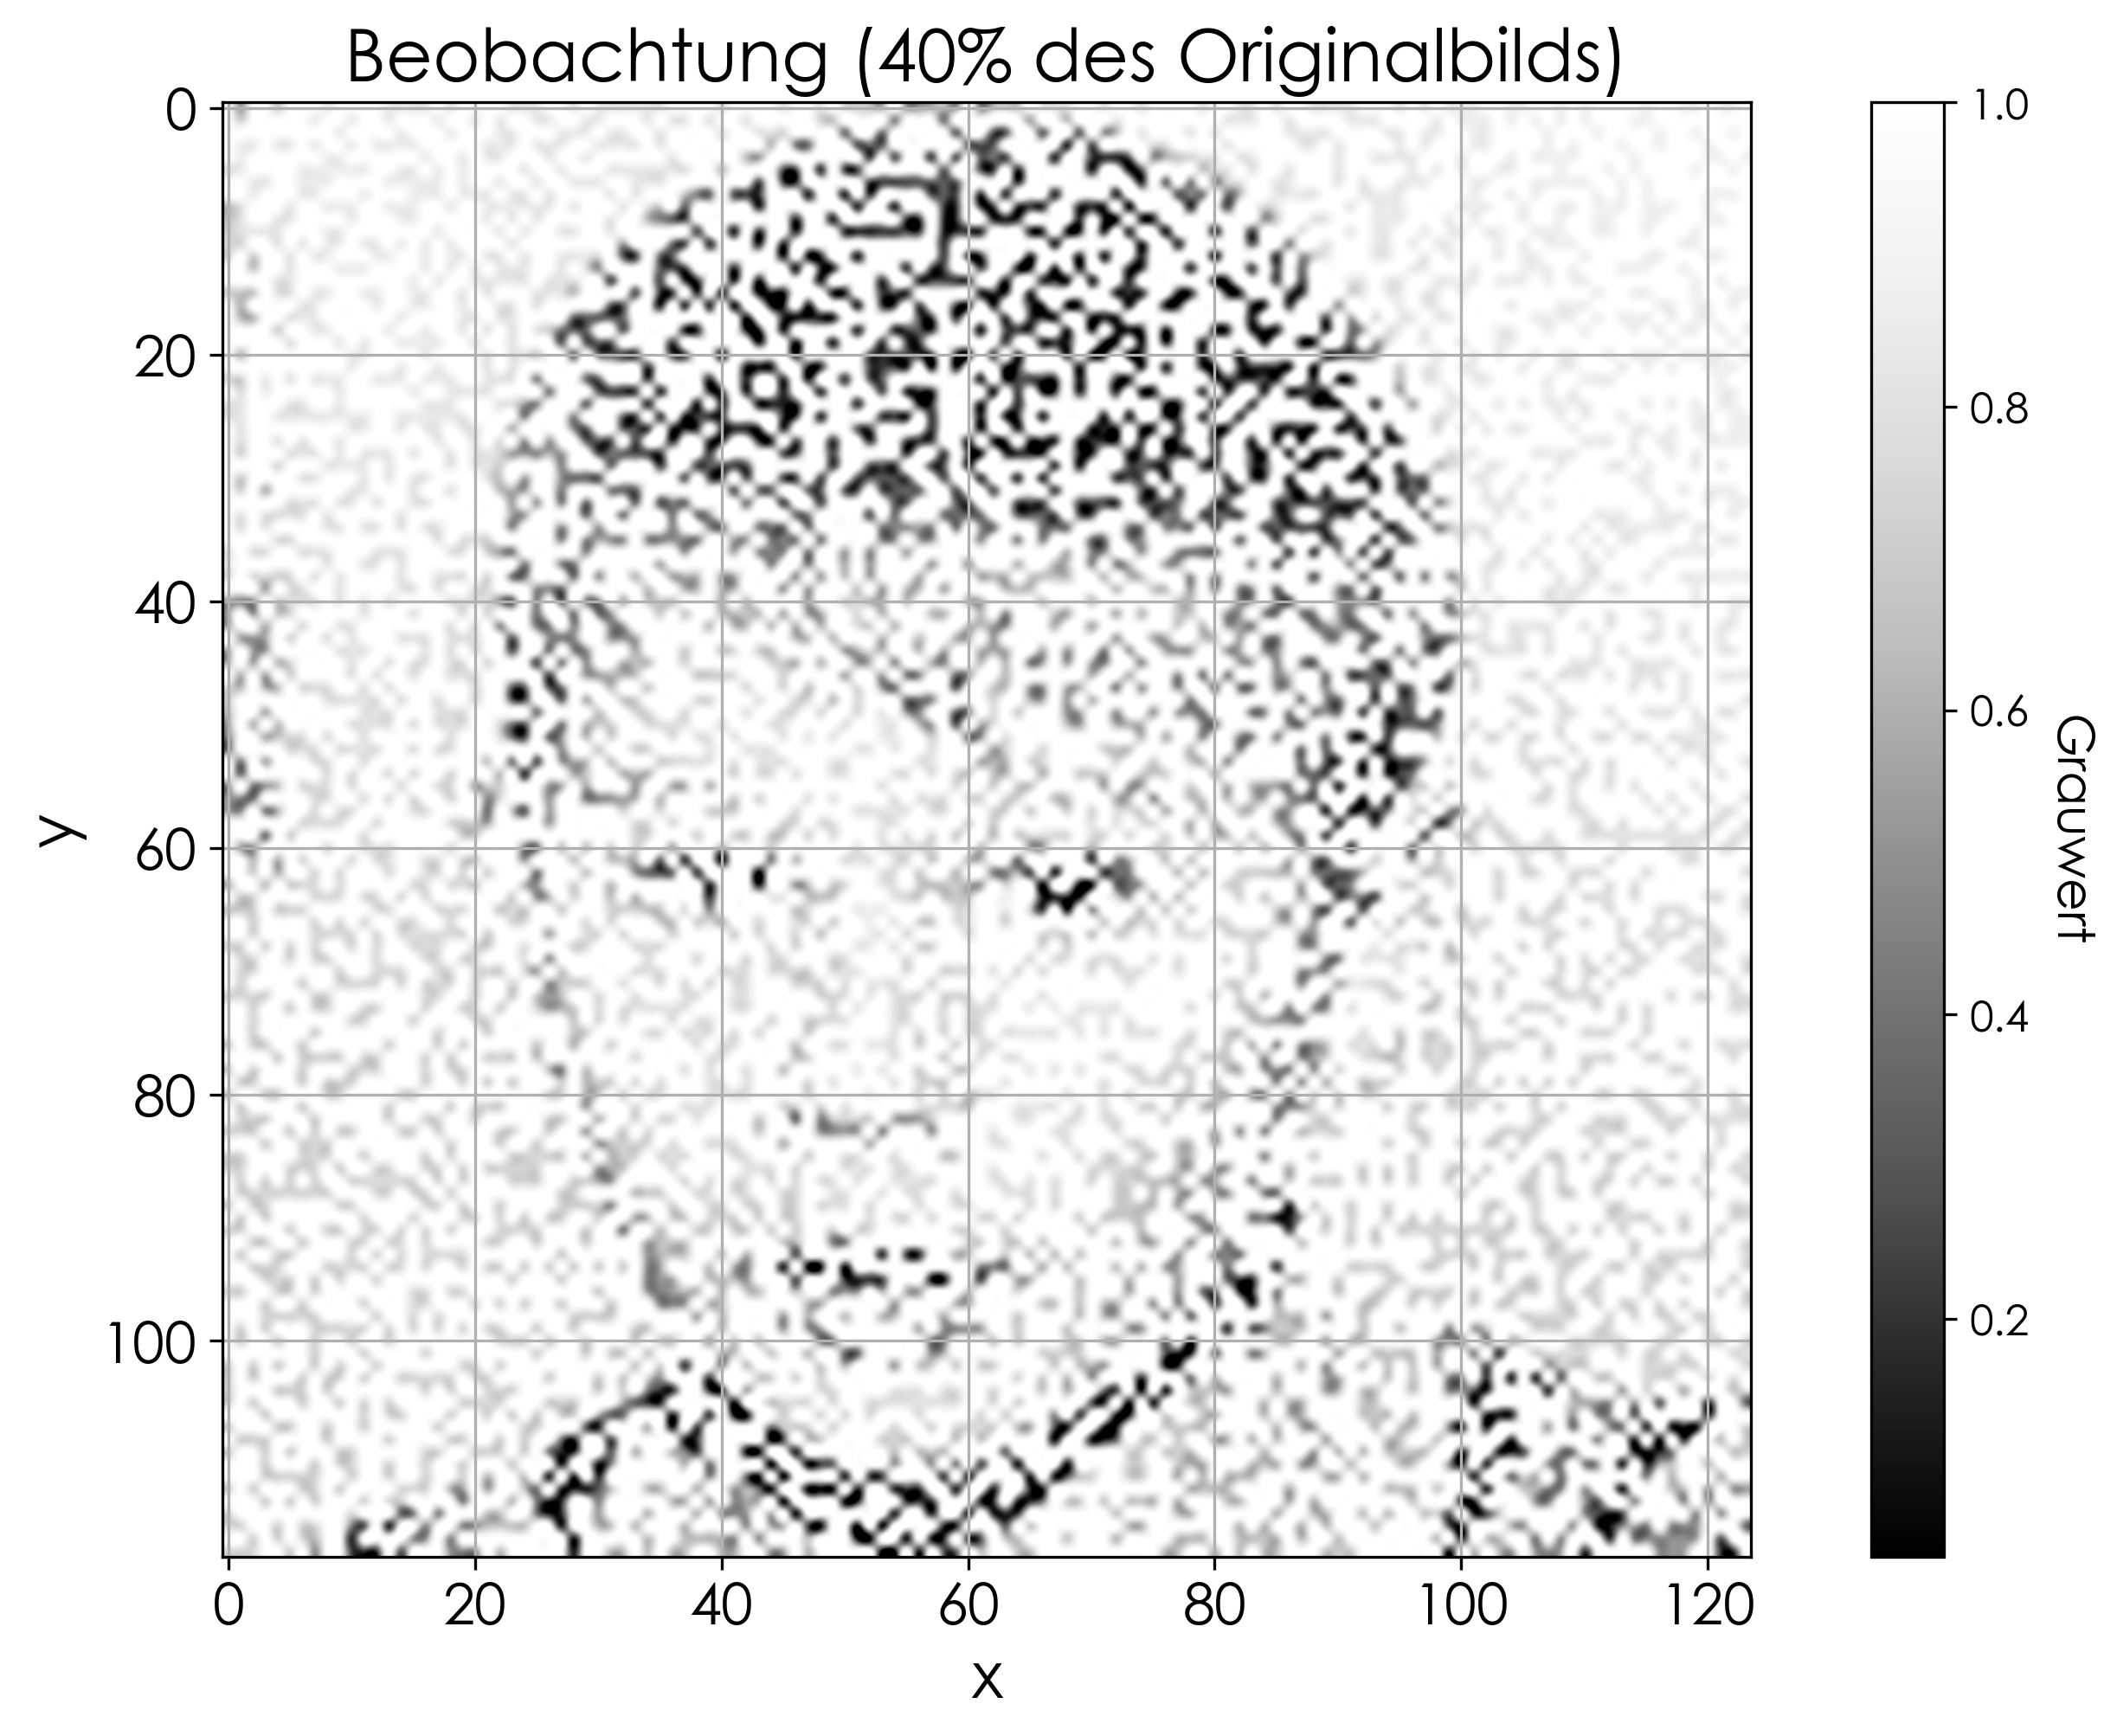
\includegraphics[scale = 0.45]{Bilder/Illustration_Kriging 40Prz Ausgangslage} 
\caption{\small{Teilweise beobachtete \glqq Realität\grqq\ nach einer Stichprobenerhebung}}
\label{Abb_Illustration_Kriging 40Prz Ausgangslage}
\end{figure} 

Abb.\,(\ref{Abb_Illustration_Kriging 40Prz Ergebnis Kriging}) zeigt die Vorhersagen des Kriging angewendet 
auf das Abbild der \glqq Realität\grqq\ nach 
Abb.\,(\ref{Abb_Illustration_Kriging 40Prz Ausgangslage}).
Durch den direkten Vergleich des linken und rechten Teilbildes 
der Abb.\,(\ref{Abb_Illustration_Kriging 40Prz Ergebnis Kriging}) 
erkennt man deutlich, dass die Berücksichtigung der räumlichen
Ähnlichkeiten mittels dieser Methode qualitativ gute Vorhersagen basierend auf den Beobachtungen 
liefert.
%\footnote{Die durch multiple lineare Regression
%gewonnene Abb.\,(\ref{Abb_Illustration_Kriging 40Prz Ergebnis OLS m Interaktion}) im Anhang \ref{AnhangPorträtfotoVorhersageRegression} 
%führt hingegen zu deutlich schlechteren Ergebnissen.}.

\begin{figure}[H] 
\centering
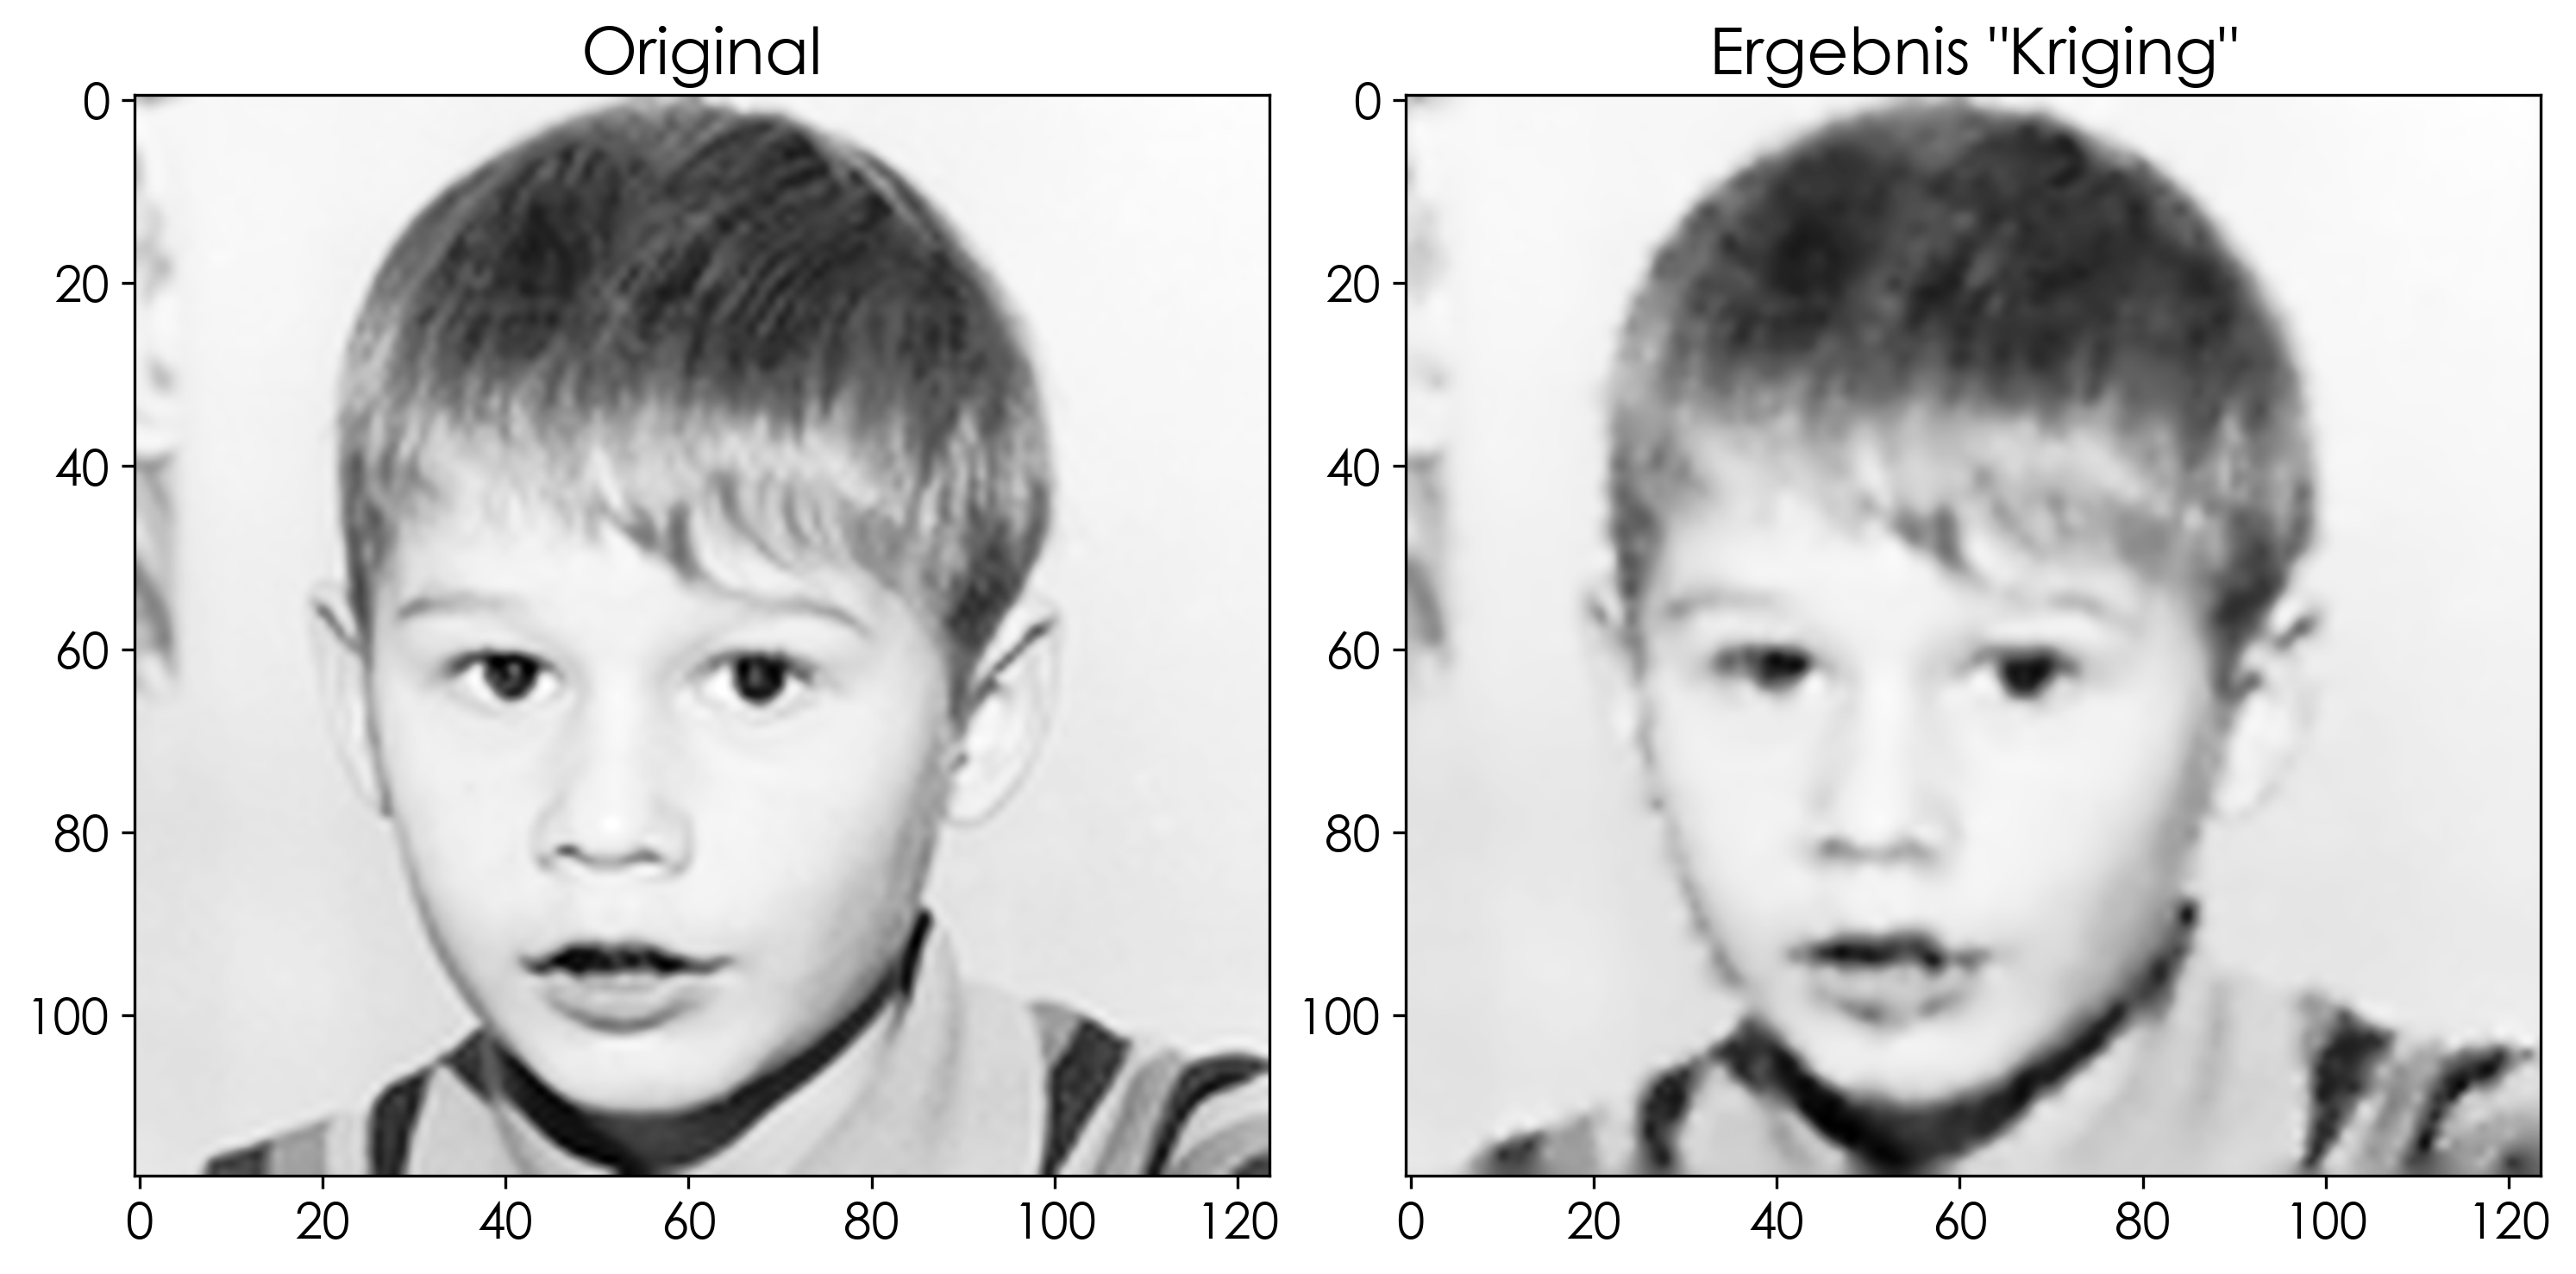
\includegraphics[scale = 0.55]{Bilder/Illustration_Kriging 40Prz Ergebnis Kriging} 
\caption{\small{Die \glqq Realität\grqq\ (links) und die aus dem Halbwissen 
mittels Kriging gewonnene Vorhersage (rechts)}}
\label{Abb_Illustration_Kriging 40Prz Ergebnis Kriging}
\end{figure} 

Dies unterstreicht die für die räumliche Statistik 
bedeutsame Beobachtung, dass räumlich näher beieinander liegende 
Beobachtungen sich ähnlicher sind als räumlich weiter entfernte 
Beobachtungen. Dieser Gedanke wird im nachfolgenden Kapitel
erneut aufgegriffen.\\
Des Weiteren verdeutlicht dieses Beispiel, weshalb Kriging 
nicht nur im Bergbau, sondern auch in anderen Disziplinen, 
etwa der Meteorologie oder der Umweltwissenschaft, eingesetzt wird.

\subsection{Gliederung dieser Arbeit}
Diese Arbeit ist wie folgt strukturiert:
\begin{itemize}[topsep=2pt,parsep=1pt,itemsep=0.5pt]
\item[$\circ$ ] Kapitel \ref{KapitelTheorie} führt in die 
theoretischen Grundlagen der räumlichen Analyse ein. Hierbei werden 
neben den grundlegenden mathematischen Begriffen auch die gängigen 
Methoden der Geostatistik und die Kriging-Gleichungen aufgeführt.  
\item[$\circ$ ] Kapitel \ref{KapitelDatenanalyse} widmet sich 
dem Themengebiet Feinstaub, erläutert die Struktur der untersuchten Daten 
und beschreibt die vorgenommenen Schritte der Datenbereinigung.
\item[$\circ$ ] In Kapitel \ref{KapitelDatenauswertung} werden 
die gewählte Herangehensweise und die Ergebnisse 
dieser Arbeit dargelegt und in den Kontext verwandter Arbeiten gebracht.
\item[$\circ$ ] Im Kapitel
 \ref{KapitelDatenauswertung_Diskussion} werden die
 Ergebnisse diskutiert und Perspektiven für vertiefende, weitere 
 Untersuchungen skizziert. Diese umfassen Analysen, 
die aufgrund der Vorgaben der Prüfungsordnung bezüglich Bearbeitungszeit und
maximaler Seitenzahl einer Bachelorarbeit nicht mehr berücksichtigt werden 
konnten\footnote{Es ist eine Bearbeitungszeit von 11 Wochen und 
eine maximale Seitenzahl von 50 vorgegeben.}.
\item[$\circ$ ] In den Anhang wurden diejenigen 
Überlegungen ausgelagert, die den Lesefluss im Hauptteil behindert 
hätten, gleichwohl zu wichtig sind, um einfach weggelassen zu werden.  
\end{itemize}
